\chapter{Architecture of Cloud-SAP}

\chapterintro{This chapter introduces architecture of Cloud-SAP, Platform-as-a-Service model that aims to satisfy requirements introduced in first chapter.}

\section{Introduction}

One can notice that elements that yields a solution for a problem stated in first chapter, which is ensuring that users' application provide appropriate Quality-of-Service for its customers, were introduced in previous chapters:
\begin{itemize}
	\item scalability - ability to improve application performance by enriching 
	\item adaptivity - ability to adapt (i.e. scale) appropriately to current usage pattern
	\item inter-cloud awareness - ability to cooperate with different cloud provider to supply application with extra resources
\end{itemize}

To begin with, different scalability models were introduced. Noticeably, they operated at different layers: 
\begin{itemize}
	\item application platform tuning
	\item single-server level (vertical scaling)
	\item multi-server level (horizontal scaling) 
	\item inter-cloud level (scaling out across different cloud-providers, concept introduced in previous chapter)
\end{itemize}
Consequently, it is expected that proposed solution's architecture reflects that multi-layered model, which, as Table \ref{tab:cloud-providers-scaling} illustrates, hasn't been yet introduced to the marked. Additionally, each layer has to be characterized by an ability to adapt to a given application usage. As previous chapter stated, this can be achieved by adding a elasticity controller to each layer. This observation is a foundation of proposed architecture.

One of the first models that ensured system adaptivity is an autonomic component, concept based on a feed-back loop, initially proposed by IBM \cite{IBM06}. Figure \ref{ch5:autonomic-component} depicts that architecture. 

\begin{figure}[!ht]
  \begin{center}
    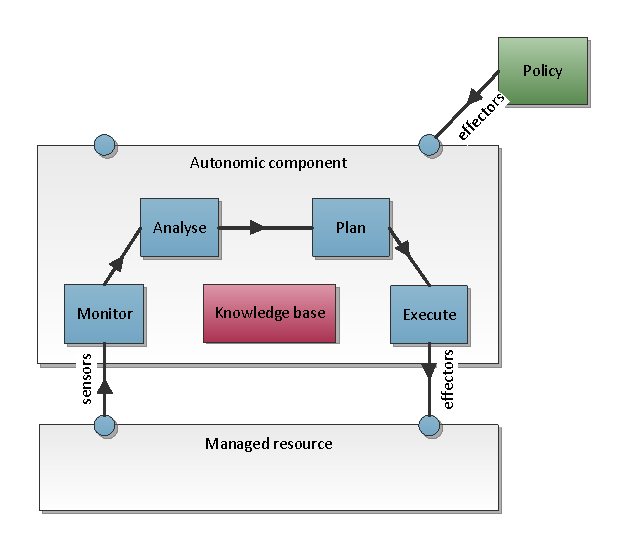
\includegraphics{chapter-5/autonomic-component}
  \end{center}
  \caption{Autonomic component}
  \label{ch5:autonomic-component}
\end{figure}

Since designed platform operates on multiple layers, we can extend that model by using concept of a multi-hierarchical autonomic system \cite{LiWoZh05}. Figure \ref{ch5:hierarchical-autonomic-system} illustrates that hierarchy, were each level represents a different perspective at application scaling. Using terminology characteristic to a autonomic system, first three hierarchy levels (application tuning, single-server, multi-server) are centralized and controlled by single elasticity controller at each level, while the last inter-cloud level is a decentralized one - each cloud instance is fully independent.

\begin{figure}[!ht]
  \begin{center}
    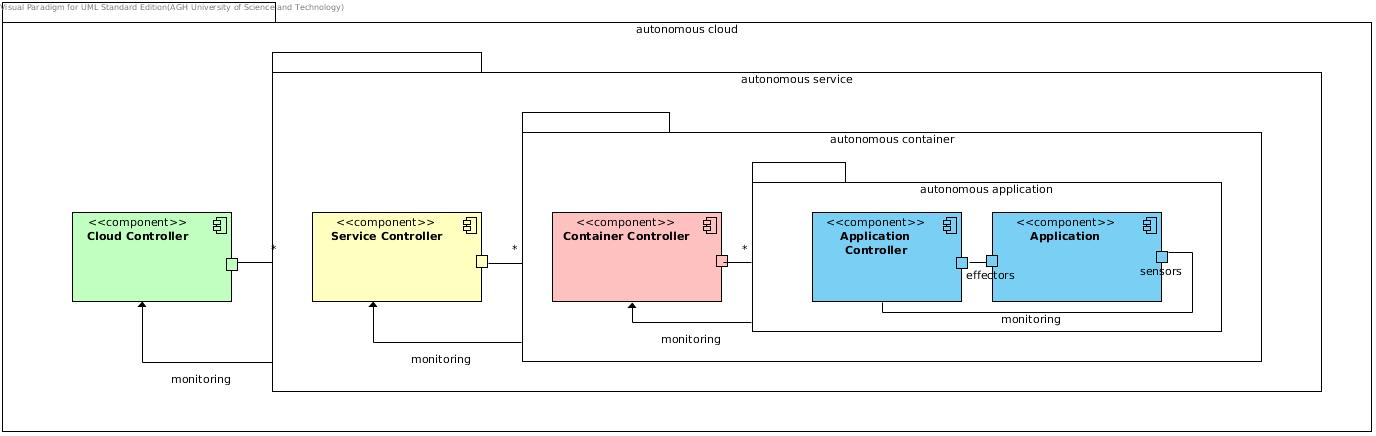
\includegraphics{chapter-5/hierarchical-autonomic-system}
  \end{center}
  \caption{Hierarchical autonomic system}
  \label{ch5:hierarchical-autonomic-system}
\end{figure}

As \cite{IBM06} states, each autonomic component has modules that are responsible for:
\begin{itemize}
	\item monitoring
	\item analysis
	\item planning
	\item action execution
\end{itemize}

While the managed component has:
\begin{itemize}
	\item sensors
	\item effectors
\end{itemize}

Due to the hierarchy of our architecture, each level manages an underlying autonomic component, while being managed by an upper layer at the same time. This lead us to observation that they are autonomic components and managed components at the same time. Remaining of this chapter discusses in detail each layer taking into account that observation.

